
\documentclass[crop,tikz]{standalone}
\usepackage[utf8]{inputenc}
\usepackage{tikz}
\usepackage{pgfplots}
\pgfplotsset{compat=newest}
\usepgfplotslibrary{groupplots}
\begin{document}

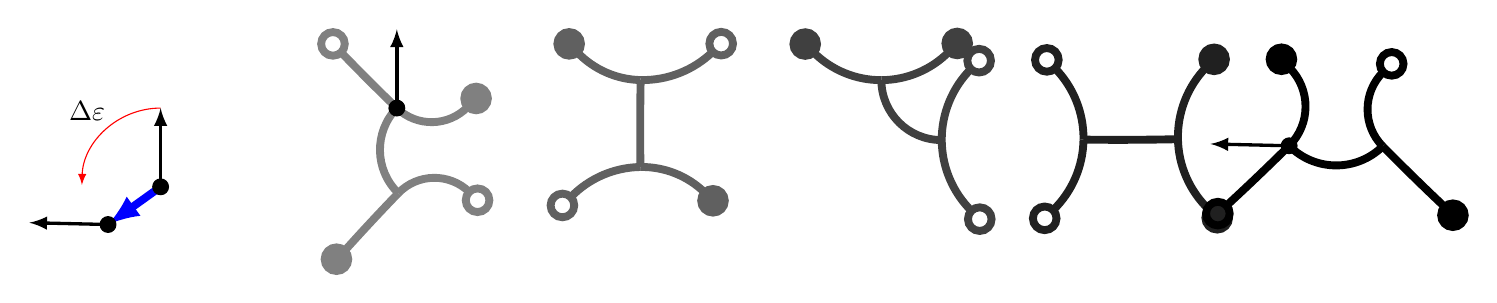
\begin{tikzpicture}[scale=1]%%%% POSE 0
\begin{scope}[xshift=0 cm]

\def\col{black!50.0}
\def\lw{1mm}
\def\alpi{2.000000}
\def\beti{90.000000}
\def\gam{90.000000}
\def\alpii{2.000000}
\def\betii{90.000000}
\def\gamh{45.000000}

\def\eps{90.000006}
\def\ci{44.000006}
\def\cii{135.000006}
\def\ciii{316.000006}
\def\civ{225.000006}

\def\ri{28.647887}
\def\rii{0.636620}
\def\rg{0.763944}
\def\riii{28.647890}
\def\riv{0.636620}

\path (0.000000, -0.000000)coordinate(F1);

\draw[\col, line width=\lw] (F1)arc(180+\ci:180+\ci+\alpi:\ri)coordinate(OM);
\draw[\col, line width=\lw] (OM)arc(180+\ci+\alpi:180+\ci+\alpi+\beti:\rii)coordinate(F2);
\draw[\col, line width=\lw] (OM)arc(90+\ci+\alpi:90+\ci+\alpi+\gam:\rg)coordinate(UM);
\draw[\col, line width=\lw] (UM)arc(\gam+\ci+\alpi:\gam+\ci+\alpi+\alpii:\riii)coordinate(F3);
\draw[\col, line width=\lw] (UM)arc(\gam+\ci+\alpi:\gam+\ci+\alpi-\betii:\riv)coordinate(F4);

\draw[\col, line width=\lw] (F1)++(134.000006 :.15) circle(.15);
\draw[\col, line width=\lw, fill] (F2)++(45.000006 :.15) circle(.15);
\draw[\col, line width=\lw, fill] (F3)++(226.000006 :.15) circle(.15);
\draw[\col, line width=\lw] (F4)++(315.000006 :.15) circle(.15);
\path (OM)coordinate(start); 
\draw[very thick, -latex] (OM)--++(\eps:1); 
\draw[fill] (OM)circle(.1); 
\end{scope} 



%%%% POSE 1
\begin{scope}[xshift=3 cm]

\def\col{black!62.5}
\def\lw{1mm}
\def\alpi{45.000000}
\def\beti{45.000000}
\def\gam{2.000000}
\def\alpii{45.000000}
\def\betii{45.000000}
\def\gamh{1.000000}

\def\eps{89.380663}
\def\ci{43.880663}
\def\cii{133.880663}
\def\ciii{314.880663}
\def\civ{224.880663}

\def\ri{1.145916}
\def\rii{1.283663}
\def\rg{31.655473}
\def\riii{1.259503}
\def\riv{1.145920}

\path (0.000000, -0.000000)coordinate(F1);

\draw[\col, line width=\lw] (F1)arc(180+\ci:180+\ci+\alpi:\ri)coordinate(OM);
\draw[\col, line width=\lw] (OM)arc(180+\ci+\alpi:180+\ci+\alpi+\beti:\rii)coordinate(F2);
\draw[\col, line width=\lw] (OM)arc(90+\ci+\alpi:90+\ci+\alpi+\gam:\rg)coordinate(UM);
\draw[\col, line width=\lw] (UM)arc(\gam+\ci+\alpi:\gam+\ci+\alpi+\alpii:\riii)coordinate(F3);
\draw[\col, line width=\lw] (UM)arc(\gam+\ci+\alpi:\gam+\ci+\alpi-\betii:\riv)coordinate(F4);

\draw[\col, line width=\lw, fill] (F1)++(133.880663 :.15) circle(.15);
\draw[\col, line width=\lw] (F2)++(43.880663 :.15) circle(.15);
\draw[\col, line width=\lw] (F3)++(224.880663 :.15) circle(.15);
\draw[\col, line width=\lw, fill] (F4)++(314.880663 :.15) circle(.15);
\end{scope} 



%%%% POSE 2
\begin{scope}[xshift=6 cm]

\def\col{black!75.0}
\def\lw{1mm}
\def\alpi{45.000000}
\def\beti{45.000000}
\def\gam{90.000000}
\def\alpii{45.000000}
\def\betii{45.000000}
\def\gamh{45.000000}

\def\eps{135.225449}
\def\ci{45.225449}
\def\cii{135.225449}
\def\ciii{45.225449}
\def\civ{315.225449}

\def\ri{1.215098}
\def\rii{1.215151}
\def\rg{0.763943}
\def\riii{1.273235}
\def\riv{1.273237}

\path (0.000000, -0.000000)coordinate(F1);

\draw[\col, line width=\lw] (F1)arc(180+\ci:180+\ci+\alpi:\ri)coordinate(OM);
\draw[\col, line width=\lw] (OM)arc(180+\ci+\alpi:180+\ci+\alpi+\beti:\rii)coordinate(F2);
\draw[\col, line width=\lw] (OM)arc(90+\ci+\alpi:90+\ci+\alpi+\gam:\rg)coordinate(UM);
\draw[\col, line width=\lw] (UM)arc(\gam+\ci+\alpi:\gam+\ci+\alpi+\alpii:\riii)coordinate(F3);
\draw[\col, line width=\lw] (UM)arc(\gam+\ci+\alpi:\gam+\ci+\alpi-\betii:\riv)coordinate(F4);

\draw[\col, line width=\lw, fill] (F1)++(135.225449 :.15) circle(.15);
\draw[\col, line width=\lw, fill] (F2)++(45.225449 :.15) circle(.15);
\draw[\col, line width=\lw] (F3)++(-44.774551 :.15) circle(.15);
\draw[\col, line width=\lw] (F4)++(405.225449 :.15) circle(.15);
\end{scope} 



%%%% POSE 3
\begin{scope}[xshift=9 cm]

\def\col{black!87.5}
\def\lw{1mm}
\def\alpi{45.000000}
\def\beti{45.000000}
\def\gam{2.000000}
\def\alpii{45.000000}
\def\betii{45.000000}
\def\gamh{1.000000}

\def\eps{179.725424}
\def\ci{134.225424}
\def\cii{224.225424}
\def\ciii{45.225424}
\def\civ{315.225424}

\def\ri{1.273240}
\def\rii{1.273241}
\def\rg{34.377459}
\def\riii{1.273236}
\def\riv{1.273235}

\path (0.042510, -2.002883)coordinate(F1);

\draw[\col, line width=\lw] (F1)arc(180+\ci:180+\ci+\alpi:\ri)coordinate(OM);
\draw[\col, line width=\lw] (OM)arc(180+\ci+\alpi:180+\ci+\alpi+\beti:\rii)coordinate(F2);
\draw[\col, line width=\lw] (OM)arc(90+\ci+\alpi:90+\ci+\alpi+\gam:\rg)coordinate(UM);
\draw[\col, line width=\lw] (UM)arc(\gam+\ci+\alpi:\gam+\ci+\alpi+\alpii:\riii)coordinate(F3);
\draw[\col, line width=\lw] (UM)arc(\gam+\ci+\alpi:\gam+\ci+\alpi-\betii:\riv)coordinate(F4);

\draw[\col, line width=\lw] (F1)++(224.225424 :.15) circle(.15);
\draw[\col, line width=\lw] (F2)++(134.225424 :.15) circle(.15);
\draw[\col, line width=\lw, fill] (F3)++(-44.774576 :.15) circle(.15);
\draw[\col, line width=\lw, fill] (F4)++(405.225424 :.15) circle(.15);
\end{scope} 



%%%% POSE 4
\begin{scope}[xshift=12 cm]

\def\col{black!100.0}
\def\lw{1mm}
\def\alpi{2.000000}
\def\beti{90.000000}
\def\gam{90.000000}
\def\alpii{2.000000}
\def\betii{90.000000}
\def\gamh{45.000000}

\def\eps{178.668944}
\def\ci{132.668944}
\def\cii{223.668944}
\def\ciii{44.668944}
\def\civ{313.668944}

\def\ri{31.511593}
\def\rii{0.700282}
\def\rg{0.840338}
\def\riii{31.512678}
\def\riv{0.667284}

\path (-0.755740, -1.945806)coordinate(F1);

\draw[\col, line width=\lw] (F1)arc(180+\ci:180+\ci+\alpi:\ri)coordinate(OM);
\draw[\col, line width=\lw] (OM)arc(180+\ci+\alpi:180+\ci+\alpi+\beti:\rii)coordinate(F2);
\draw[\col, line width=\lw] (OM)arc(90+\ci+\alpi:90+\ci+\alpi+\gam:\rg)coordinate(UM);
\draw[\col, line width=\lw] (UM)arc(\gam+\ci+\alpi:\gam+\ci+\alpi+\alpii:\riii)coordinate(F3);
\draw[\col, line width=\lw] (UM)arc(\gam+\ci+\alpi:\gam+\ci+\alpi-\betii:\riv)coordinate(F4);

\draw[\col, line width=\lw] (F1)++(222.668944 :.15) circle(.15);
\draw[\col, line width=\lw, fill] (F2)++(133.668944 :.15) circle(.15);
\draw[\col, line width=\lw, fill] (F3)++(-45.331056 :.15) circle(.15);
\draw[\col, line width=\lw] (F4)++(403.668944 :.15) circle(.15);
\path (OM)coordinate(end); 
\draw[very thick, -latex] (OM)--++(\eps:1); 
\draw[fill] (OM)circle(.1); 
\end{scope} 



\draw[line width=1mm, latex-, blue] (end)++(-15,-1)coordinate(end_)--($(start)+(-3,-1)$)coordinate(start_) ;
\draw[-latex, red] (start_)++(90:1)arc(90:178.668944184:1);
\path (start_)++(134.33447209212488:1)node[anchor=314.3344720921249]{$\Delta \varepsilon$};\draw[fill] (start_)circle(.1); 
\draw[very thick, -latex] (start_)--++(90:1); 
\draw[fill] (end_)circle(.1); 
\draw[very thick, -latex] (end_)--++(178.668944184:1); 
% This file was created by matplotlib2tikz v0.6.18.

\end{tikzpicture}
%% End matplotlib2tikz content %% 
\end{document}